\intro{}




\section{Divisione}



\defn{Divisibilità}{
Se $a$ e $b$ sono numeri interi con $a \neq 0$, si dice che $a$ divide $b$ se esiste un intero $c$ tale che $b = ac$. 

Quando $a$ divide $b$, si dice che $a$ è un divisore di $b$ e che $b$ è un multiplo di $a$. La notazione $a \mid b$ indica che $a$ divide $b$. Si scrive $a \nmid b$ quando $a$ non divide $b$.
}



\thm{Proprietà della divisibilità}{
Siano $a,b,c \in \mathbb{Z}$, $a \neq 0$. Allora:
\begin{itemize}
    \item $a \mid b$ e $a \mid c \implies a \mid (b+c)$
    \item $a \mid b \implies a \mid bc$ $\forall c \in \mathbb{Z}$
    \item $a \mid b$ e $b \mid c \implies a \mid c$
\end{itemize}
}

\cor{
Siano $a,b,c \in \mathbb{Z}$, $a \neq 0$, $a \mid b$, $a \mid c$. Allora $a \mid (mb+nc)$ $\forall m,n \in \mathbb{Z}$.
}



\thm{Divisione euclidea}{
Per ogni $a,b \in \mathbb{Z}$, $b \neq 0$, esiste un'unica coppia $q,r \in \mathbb{Z}$ tale che:
\[
a = bq + r, \quad 0 \leq r < |b|
\]
($a$=dividendo, $b$=divisore, $q$=quoziente, $r$=resto).
}
















\exm{Teorema della divisione euclidea (esistenza e unicità di quoziente e resto)}{

Dimostriamo prima l'esistenza degli interi \(q\) ed \(r\), poi la loro unicità. 


L'enunciato standard richiede \(b\neq 0\) e impone \(0\le r<|b|\). Per semplificare la prova, è comodo ridursi al caso \(b>0\) e (per l'esistenza) \(a\ge 0\): il valore assoluto su \(b\) serve proprio a gestire anche \(b<0\). 


\medskip

\textbf{Riduzione al caso \(b>0\).}
Se \(b<0\), poniamo \(b'=-b>0\). Allora
\[
a=bq+r \quad \Longleftrightarrow \quad a=b'(-q)+r,
\]
e la condizione \(0\le r<|b|\) coincide con \(0\le r<b'\). Quindi è sufficiente dimostrare il teorema per \(b>0\). 

\medskip

\textbf{(1) Esistenza (per induzione su \(a\ge 0\)).}
Fissiamo \(b>0\). Dimostriamo per induzione su \(a\in\mathbb{N}\) che esistono \(q,r\in\mathbb{Z}\) tali che
\[
a=bq+r \qquad \text{con} \qquad 0\le r<b.
\] 

\begin{itemize}
\item \textbf{Caso base \(a=0\).} Basta scegliere \(q=0\) e \(r=0\). Infatti \(0=b\cdot 0+0\) e \(0\le 0<b\). 


\item \textbf{Passo induttivo.} Sia \(a>0\) e supponiamo vera la proprietà per tutti gli interi \(a'<a\) (in particolare per \(a-b\) quando ha senso). Mostriamo che vale per \(a\).
\end{itemize}

Distinguiamo due casi. 

\begin{itemize}
\item \textbf{Se \(a<b\).} Prendiamo \(q=0\) e \(r=a\). Allora \(a=b\cdot 0 + a\) e \(0\le a<b\). 

\item \textbf{Se \(a\ge b\).} Allora \(a-b\ge 0\) e per ipotesi induttiva esistono \(q'\) e \(r'\) tali che
\[
a-b = bq' + r' \qquad \text{con} \qquad 0\le r' < b.
\]
Sommiamo \(b\) a entrambi i membri:
\[
a = b(q'+1) + r'.
\]
Quindi ponendo \(q=q'+1\) e \(r=r'\) otteniamo la forma richiesta con \(0\le r<b\). 
\end{itemize}

Questo conclude la parte di esistenza per \(a\ge 0\) e \(b>0\).

 l'induzione costruisce \(a\) sottraendo \(b\) tante volte finché si scende sotto \(b\). Quel “valore finale” è il resto \(r\), mentre quante sottrazioni sono state fatte corrisponde al quoziente \(q\). 

\medskip

\textbf{(2) Unicità.}
Supponiamo che esistano due coppie \((q,r)\) e \((q',r')\) tali che
\[
a=bq+r,\qquad 0\le r<b,
\]
\[
a=bq'+r',\qquad 0\le r'<b.
\]
Sottraendo membro a membro otteniamo
\[
b(q-q') = r'-r.
\] 

Dalle disuguaglianze su \(r\) e \(r'\) segue che \(|r'-r|<b\). Quindi \(|b|\cdot |q-q'| = |r'-r| < b\), cioè \(|q-q'|<1\). Essendo \(q-q'\in\mathbb{Z}\), l'unica possibilità è \(q-q'=0\), dunque \(q=q'\), e di conseguenza anche \(r=r'\). 

}







\section{Aritmetica dell'orologio}

L'aritmetica modulare (o \virgolette{aritmetica dell'orologio}) descrive situazioni in cui, raggiunto un certo valore \(n\), si \virgolette{riparte da capo}: i numeri vengono considerati a meno di multipli di \(n\).
L'impostazione moderna delle congruenze (e quindi dell'aritmetica modulare) viene fatta risalire a Gauss, in particolare alla sua opera \emph{Disquisitiones Arithmeticae} (1801).

\rmkb{
L'idea dell'orologio è una visualizzazione del fatto che due numeri sono considerati \virgolette{uguali} se differiscono di un giro completo, cioè di un multiplo di \(n\). Per esempio, in un orologio a 12 ore, 15 e 3 indicano la stessa posizione perché \(15-3=12\), cioè un giro completo.
}

\defn{Congruenza modulo \(n\)}{
Sia \(n\in\mathbb{Z}\) con \(n>0\). Per \(a,b\in\mathbb{Z}\) si dice che \(a\) è \textbf{congruente} a \(b\) \textbf{modulo \(n\)}, e si scrive
\[
a \equiv b \pmod n,
\]
se e solo se \(n\mid (a-b)\), cioè se esiste \(k\in\mathbb{Z}\) tale che \(a-b=kn\).


 \(a\equiv b\pmod n\) significa che, dividendo \(a\) e \(b\) per \(n\), si ottiene lo stesso resto (quindi corrispondono alla stessa \virgolette{tacca} sull'orologio a \(n\) posizioni). È equivalente a dire che da \(b\) si arriva ad \(a\) facendo un certo numero di giri completi di ampiezza \(n\).





}





Nel linguaggio dell'orologio a \(n\) tacche, lavorare \virgolette{modulo \(n\)} significa identificare tutte le posizioni che differiscono per un numero intero di giri completi.


\begin{center}
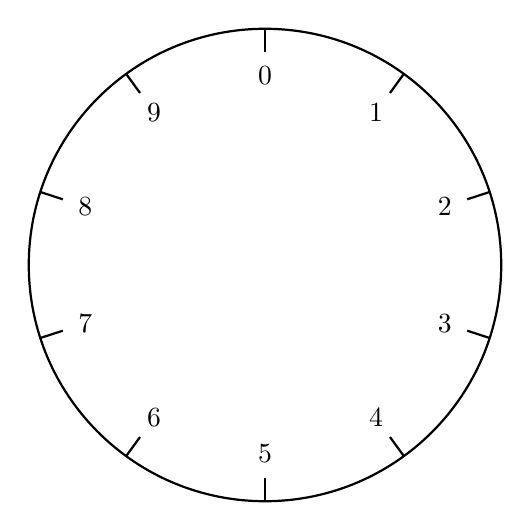
\begin{tikzpicture}[scale=3]
    % Cerchio principale
    \draw[thick] (0,0) circle(1);

    % Posizionamento dei numeri (esempio con n=10)
    \foreach \i in {0,1,2,3,4,5,6,7,8,9} {
        \node at ({90-\i*36}:0.8) {\i};
    }

    % Linee delle tacche
    \foreach \i in {0,1,...,9} {
        \draw[thick] ({90-\i*36}:0.9) -- ({90-\i*36}:1);
    }
\end{tikzpicture}
\end{center}

\rmkb{
Nella figura si è scelto \(n=10\) solo per avere un disegno semplice: concettualmente è lo stesso per qualunque \(n>0\). L'operazione \(a \bmod n\) restituisce la \virgolette{posizione} finale dopo aver fatto avanzare di \(a\) passi su un orologio con \(n\) tacche, cioè il resto \(r\) della divisione euclidea \(a=nq+r\) con \(0\le r<n\).
}

























\section{Operazioni  e Congruenze}

\subsection*{Interpretazione geometrica: l'Aritmetica dell'Orologio}

Possiamo visualizzare le operazioni aritmetiche su \(\mathbb{Z}_n = \{0, 1, \dots, n-1\}\) come movimenti su un quadrante con \(n\) tacche.

\begin{itemize}
    \item \textbf{Scorrimento in senso orario (+1):}
    Una mossa +1 consiste nello spostarsi dalla tacca corrente alla successiva in senso orario. 
    \[
    x \mapsto (x + 1) \bmod n.
    \]
    \emph{Caso speciale:} Se siamo sulla tacca \(n-1\), il passo successivo ci riporta a 0. Dunque, in questo sistema, 0 è il successore di \(n-1\).

    \item \textbf{Scorrimento in senso antiorario (-1):}
    Una mossa -1 consiste nello spostarsi dalla tacca corrente alla precedente in senso antiorario.
    \[
    x \mapsto (x - 1) \bmod n.
    \]
    \emph{Caso speciale:} Se siamo sulla tacca 0, il passo precedente ci porta a \(n-1\).
\end{itemize}

La funzione determinata dalle mosse \(+1\) è una funzione \textbf{biunivoca} \(f: \mathbb{Z}_n \to \mathbb{Z}_n\).

\begin{esempio}
Consideriamo l'insieme \(\mathbb{Z}_{10} = \{0, 1, 2, \dots, 9\}\).

\strategia{Analizziamo i movimenti su un orologio con \(n=10\) tacche (\(\mathbb{Z}_{10}\)). Ricordiamo che operare modulo 10 significa considerare solo l'ultima cifra del risultato (se positivo) o tornare indietro ciclicamente (se negativo).}

\begin{itemize}
    \item Partendo da \(7\), passo \(+1\): \(7 + 1 = 8\).
    \item Partendo da \(7\), passo \(-1\): \(7 - 1 = 6\).
    \item Partendo da \(9\), passo \(+1\): si ha \(9+1=10\), ma \(10 \equiv 0 \pmod{10}\). Quindi arriviamo a \(0\).
    \item Partendo da \(2\), passo \(-1\): \(2 - 1 = 1\).
    \item Partendo da \(0\), passo \(-1\): matematicamente \(0-1=-1\). Modulo 10, \(-1 \equiv 9 \pmod{10}\), quindi arriviamo a \(9\).
\end{itemize}
\end{esempio}


\defn{Residuo e Insieme \(\mathbb{Z}_n\)}{
Siano \( a, n \in \mathbb{Z} \) con \( n > 1 \).
Il \textbf{residuo} di \( a \) modulo \( n \), indicato come \( a \bmod n \), è il resto della divisione euclidea di \( a \) per \( n \) (quindi l'unico intero \(r\) tale che \(a = nq + r\) con \(0 \le r < n\)).

L'insieme
\[
\mathbb{Z}_n = \{0, 1, 2, \dots, n-1\}
\]
è chiamato \textbf{insieme delle classi di resto} (o dei residui) modulo \( n \).

\rmkb{
\textbf{Nota terminologica:} Spesso si usa l'espressione "ridurre \(a\) modulo \(n\)" per indicare l'operazione di calcolo del resto. Quando il modulo \(n\) è chiaro dal contesto, si omette e si parla semplicemente di residuo.
}
}

\defn{Operazioni in \(\mathbb{Z}_n\)}{
Definiamo la somma (\( +_n \)) e il prodotto (\( \cdot_n \)) modulo \( n \) per ogni coppia \( a, b \in \mathbb{Z} \) come:
\[
a +_n b = (a + b) \bmod n
\]
\[
a \cdot_n b = (a \cdot b) \bmod n
\]


}
\medskip

\rmkb{
Il pedice \(n\) nelle operazioni (\(+_n, \cdot_n\)) viene spesso omesso quando non c'è ambiguità, scrivendo direttamente \(+\) e \(\cdot\) tra classi di resto.
}

\thm{Chiusura di \(\mathbb{Z}_n\)}{
L'insieme \(\mathbb{Z}_n\), equipaggiato con le operazioni \( +_n \) e \( \cdot_n \), è \textbf{chiuso}.
Ovvero, per ogni \( a, b \in \mathbb{Z}_n \):
\[
a +_n b \in \mathbb{Z}_n \quad \text{e} \quad a \cdot_n b \in \mathbb{Z}_n.
\]
}

\propi{Proprietà dell'aritmetica modulare}{
\item \textbf{Compatibilità con somma e prodotto:}
\[
(a + b) \bmod n = \big((a \bmod n) + (b \bmod n)\big) \bmod n
\]
\[
(a \cdot b) \bmod n = \big((a \bmod n) \cdot (b \bmod n)\big) \bmod n
\]
}

\subsection{La Relazione di Congruenza}

\defn{Relazione di Congruenza}{
Sia \( n \in \mathbb{Z}, n > 0 \). Definiamo la relazione binaria \( \mathcal{R} \) su \( \mathbb{Z} \) nel modo seguente:
\[
a \mathrel{\mathcal{R}} b \iff (a \bmod n) = (b \bmod n).
\]
In altre parole, \(a\) è in relazione con \(b\) se e solo se, divisi per \(n\), danno lo stesso resto.
Questa relazione coincide con la congruenza definita in precedenza:
\[
a \mathrel{\mathcal{R}} b \iff n \mid (a - b) \iff a \equiv b \pmod n.
\]


}


\rmkb{
Questa definizione mostra che la congruenza modulo \(n\) è una \textbf{relazione di equivalenza}. Essa partiziona l'insieme dei numeri interi \(\mathbb{Z}\) esattamente nelle \(n\) classi rappresentate dagli elementi di \(\mathbb{Z}_n\).
}















\thmr{Congruenza modulo \(n\) come relazione di equivalenza}{thm:cong_equiv}{
Sia \( n \in \mathbb{Z} \) con \( n > 1 \). La relazione di congruenza modulo \( n \) è una \textbf{relazione di equivalenza} sull'insieme degli interi \( \mathbb{Z} \).

Le classi di equivalenza distinte sono esattamente \(n\) e corrispondono ai possibili resti della divisione per \(n\):
\[
[0], [1], [2], \dots, [n-1],
\]
dove per ogni \( a \in \{0, 1, \dots, n-1\} \) la classe è definita come:
\[
[a]_n = \{m \in \mathbb{Z} \mid m \equiv a \pmod n \} = \{m \in \mathbb{Z} \mid m = a + kn, \text{ con } k \in \mathbb{Z}\}.
\]
}

\begin{thmpf}
\strategia{Per dimostrare che una relazione è di equivalenza, dobbiamo verificare tre proprietà fondamentali:
\begin{enumerate}
    \item \textbf{Riflessiva:} ogni elemento è in relazione con se stesso.
    \item \textbf{Simmetrica:} se \(a\) è in relazione con \(b\), allora \(b\) è in relazione con \(a\).
    \item \textbf{Transitiva:} se \(a\) è in relazione con \(b\) e \(b\) con \(c\), allora \(a\) è in relazione con \(c\).
\end{enumerate}
Useremo la definizione: \(a \equiv b \pmod n \iff n \mid (a-b)\), cioè \(a-b = kn\) per un intero \(k\).}

Procediamo verificando le tre proprietà:

\begin{itemize}
    \item \textbf{Riflessività.} Sia \( a \) un intero qualsiasi.
    Dobbiamo mostrare che \( a \equiv a \pmod n \), ovvero che \( n \mid (a - a) \).
    Osserviamo che:
    \[
    a - a = 0.
    \]
    Poiché \( 0 = n \cdot 0 \), si ha che \( n \mid 0 \). Pertanto \( a \equiv a \pmod n \).

    \item \textbf{Simmetria.} Siano \( a, b \in \mathbb{Z} \) tali che \( a \equiv b \pmod n \).
    Per definizione, \( n \mid (a - b) \), quindi esiste un intero \( k \) tale che:
    \[
    a - b = nk.
    \]
    Moltiplicando entrambi i membri per \(-1\), otteniamo:
    \[
    -(a - b) = -nk \implies b - a = n(-k).
    \]
    Poiché \(-k\) è un intero, segue che \( n \mid (b - a) \), e dunque \( b \equiv a \pmod n \).

    \item \textbf{Transitività.} Siano \( a, b, c \in \mathbb{Z} \) tali che \( a \equiv b \pmod n \) e \( b \equiv c \pmod n \).
    Le ipotesi implicano che \( n \mid (a - b) \) e \( n \mid (b - c) \). Esistono quindi interi \( k_1, k_2 \) tali che:
    \[
    a - b = n k_1 \quad \text{e} \quad b - c = n k_2.
    \]
    Sommando le due equazioni membro a membro:
    \[
    (a - b) + (b - c) = n k_1 + n k_2 \implies a - c = n(k_1 + k_2).
    \]
    Poiché \( k_1 + k_2 \) è un intero, \( n \mid (a - c) \). Di conseguenza, \( a \equiv c \pmod n \).
\end{itemize}

\medskip
\textbf{Descrizione delle classi di equivalenza.}
Abbiamo dimostrato che la relazione è di equivalenza, quindi partiziona \(\mathbb{Z}\) in classi disgiunte.
Dal teorema della divisione euclidea, per ogni \(m \in \mathbb{Z}\) esistono unici \(q\) ed \(r\) (con \(0 \le r < n\)) tali che \(m = nq + r\).
Questa relazione si può riscrivere come \(m - r = nq\), ovvero \(m \equiv r \pmod n\).
Ciò significa che ogni intero \(m\) appartiene alla classe di equivalenza \([r]_n\) per un unico \(r \in \{0, 1, \dots, n-1\}\).
Quindi le classi distinte sono esattamente:
\[
[0], [1], \dots, [n-1].
\]
\end{thmpf}

\section{Divisibilità}
\defn{Divisibilità}{
Siano \( (a,b)\in \ZZ \) con \(a \neq 0\). si dice che \(a\) divide \(b\) se esiste un interno \(c \in \ZZ\) tale che 
\[
b=ac
\]
In tal caso si scrive \(a \mid b\); se non esiste alcun intero \(c\), si scrive \(a \nmid b\).

Quando \(a\mid b\), si dice che \(a\) è un \textbf{divisore} di \(b\), e che \(b\) è un \textbf{multiplo} di \(a\).
\medskip

\noindent Intuitivamente \(a \mid b\) significa che \(b\) si ottiene \virgolette{ripetendo} \(a\) un numero intero di volte. 

Ad esempio \(3\mid 12\) perché \(12=3\cdot 4\), mentre \(3\nmid 10\) perché non esiste un intero \(c\) con \(10=3c\). Inoltre ogni intero non nullo divide \(0\), perché \(0=a\cdot 0\). 
}
\begin{esempio}
Siano \(n\) e \(d\) due interi positivi.
Quanti interi positivi non superiori a \(n\) sono divisibili per \(d\)?

\strategia{Vogliamo contare i multipli positivi di \(d\) che cadono nell'intervallo \(\{1,2,\dots,n\}\). Un numero è divisibile per \(d\) se e solo se è della forma \(dk\). Quindi trasformiamo il problema in un conteggio di valori possibili di \(k\).}


Gli interi positivi divisibili per \(d\) sono esattamente quelli della forma
\[
dk \qquad \text{con } k\in\mathbb{Z}_{\ge 1}.
\]
La condizione \(\,dk \le n\,\) equivale a
\[
k \le \frac{n}{d}.
\]
Dunque i valori ammessi di \(k\) sono:
\[
k=1,2,3,\dots,\left\lfloor \frac{n}{d}\right\rfloor.
\]
Ne segue che il numero di interi positivi \(\le n\) divisibili per \(d\) è
\[
\left\lfloor \frac{n}{d}\right\rfloor.
\]

\medskip
\noindent \(\left\lfloor \frac{n}{d}\right\rfloor\) è proprio il più grande intero \(k\) tale che \(dk\le n\), cioè l'ultimo multiplo di \(d\) che non supera \(n\). Tutti i multipli positivi di \(d\) fino a quel punto sono \(d,2d,3d,\dots,\left\lfloor \frac{n}{d}\right\rfloor d\).
\end{esempio}









\thm{}{Siano \(a,b,c\in\mathbb{Z}\) con \(a\neq 0\). Allora valgono le seguenti proprietà:
\begin{itemize}
    \item se \(a \mid b\) e \(a \mid c\), allora \(a \mid (b+c)\);
    \item se \(a \mid b\), allora \(a \mid bc\) per ogni \(c\in\mathbb{Z}\);
    \item se \(a \mid b\) e \(b \mid c\), allora \(a \mid c\).
\end{itemize}}







\exm{Dimostriamo le proprietà del teorema}{
    \strategia{
Usiamo sistematicamente la definizione: \(a\mid b\) significa che esiste un intero \(k\) tale che \(b=ak\).
Ogni proprietà si dimostra riscrivendo i numeri come multipli di \(a\) (o di \(b\)) e ricombinando algebricamente.
}

\begin{itemize}
    \item \textbf{Se \(a \mid b\) e \(a \mid c\), allora \(a \mid (b+c)\).}\\
    Dalle ipotesi esistono interi \(k,  \ell\) tali che 
    \[
    b = ak \ \text{e} \ c = a \ell
    \]
    Allora 
    \[
    b+c = ak + a\ell = a(k+\ell)
    \]
    Poiché \( k+\ell \in \ZZ \), segue che \( a \mid (b+c)\)
    \item \textbf{Se \(a \mid b\), allora \(a \mid bc \) per ogni intero \(c\)}.
    Dall'ipotesi esiste un intero \(k\) tale che 
    \[
    b=ak
    \]
    Moltiplichiamo per \(c\), otteniamo
    \[
    bc=(ak)c= a(kc)
    \]
    Poiché \(kc \in \mathbb{Z}\), concludiamo che \(a \mid c\)
        
\end{itemize}



}




% \begin{mydefinition}
%     Se $a$ e $b$ sono numeri interi con $a \neq 0$, si dice che $a$ divide $b$ se esiste un intero $c$ tale che $b = ac$. 
%     Quando $a$ divide $b$, si dice che $a$ è un divisore di $b$ e che $b$ è un multiplo di $a$. 
%     La notazione $a \mid b$ indica che $a$ divide $b$. Si scrive $a \nmid b$ quando $a$ non divide $b$.
% \end{mydefinition}

% \medskip

% \esempio Siano $n$ e $d$ due numeri interi positivi. Quanti interi positivi non superiori a $n$ sono divisibili per $d$?

% Gli interi positivi divisibili per $d$ sono tutti gli interi della forma $dk$, dove $k$ è un intero positivo. 
% Pertanto, il numero di interi positivi divisibili per $d$ che non sono maggiori di $n$ corrisponde al numero di interi $k$ tali che $0 \leq dk \leq n$, 
% o che $0 \leq k \leq \dfrac{n}{d}$. 
% Quindi, ci sono $\lfloor \frac{n}{d}\rfloor$ interi positivi non superiori a $n$ che sono divisibili per $d$.

% \medskip

% \begin{mytheorem}
%     Siano $a$, $b$, e $c$ interi, con $a \neq 0$. Allora:
%     \begin{itemize}
%         \item se $a \mid b$ e $a \mid c$, allora $a \mid (b+c)$;
%         \item se $a \mid b$, allora $a \mid bc$ per ogni intero $c$;
%         \item se $a \mid b$ e $b \mid c$, allora $a \mid c$.
%     \end{itemize}
% \end{mytheorem}

% \medskip

% \begin{mycorollary}
%     Siano $a$, $b$, e $c$ interi, con $a \neq 0$, tali che $a \mid b$ e $a \mid c$. 
%     Allora $a \mid (mb+nc)$ per ogni $m$ e $n$ interi.
% \end{mycorollary}
% \subsection{Divisione euclidea}
% \begin{mytheorem}
% Per ogni coppia di numeri interi $a$ e $b$ con $b \neq 0$ esiste un'unica coppia di interi $q$ e $r$ tali che 
% \[
%     a = bq+r
% \]
% Con $0 \leq r \leq |b|$, dove $|b|$ è il valore assoluto di $b$.
% Dove :
% \begin{itemize}
%     \item $a$ è il dividendo;
%     \item $b$ è il divisore;
%     \item $q$ è il quoziente;
%     \item $r$ è il resto.
% \end{itemize}
% \end{mytheorem}

% \Dimostrazione Dimostriamo prima che gli interi $q$ ed $r$ esistano e poi proviamo che sono unici. Osserviamo che è sufficiente dimostrare il teorema nel caso $a \geq 0$ e $b >0$. Infatti,
% \begin{itemize}
%     \item se $b<0$ allora $b = -b'$ e $a=(-b')q+r$ quindi $a=b'(-q)+r$ con $b'>0$
%     \item  se $a<0$ allora $a=-a'$ e "$a$ diviso $b$" è uguale a "$a'$ diviso-b" con $a'>0$
% \end{itemize}
% Assumiamo dunque $a \geq 0$ e $b>0$. Procediamo per induzione su $a$.
% \begin{itemize}
%     \item Caso base: se $a = 0$ basta prendere $q=r=0$.
%     \item Ipotesi induttiva: sia $a>0$. Supponiamo che la proprietà sia vera per tutti gli interi $a'<a$ e proviamo che la proprietà è vera per $a$.
% \end{itemize}

% Distinguiamo due casi:
% \begin{itemize}
%     \item Se $a < b$, allora è sufficiente prendere $q = 0$ e $r = a$ (con $0 \leq r < |b|$).
%     \item Se $a \geq b$, allora, per ipotesi induttiva, la proprietà è vera per i numeri $(a - b)$ e $b$, ossia esistono $q'$ e $r'$ tali che $(a - b) = bq' + r'$ con $0 \leq r' < |b|$.  
%     Allora:
%     \[
%     a = b(q' + 1) + r'.
%     \]
% \end{itemize}

% Unicità di $q$ e $r$:
% Dimostriamo ora che $q$ ed $r$ sono unici.  
% Supponiamo che valgano $a = bq + r$ e $a = bq' + r'$ con $0 \leq r, r' < |b|$.  
% Sottraendo membro a membro, si ottiene:
% \[
% b(q - q') = (r' - r).
% \]
% Dalla relazione $0 \leq r, r' < |b|$, si ha $|r' - r| < |b|$.  
% Pertanto:
% \[
% |b||q - q'| = |r' - r| \quad \text{e dunque} \quad |q - q'| < 1.
% \]
% Dato che $q$ e $q'$ sono interi, segue che $q - q' = 0$, cioè $q = q'$. Inoltre, anche $r' - r = 0$, ossia $r = r'$.  
% Quindi, $q$ ed $r$ sono unici.

% \esempio Siano $a = 17$ e $b=-3$. Allora
% \[
%     17 = (-3) \cdot (-5)+2
% \]

% \esempio Siano $a = -17$ e $b=-3$. Allora
% \[
%     -17 = (-3) \cdot (6)+1
% \]
% \section{Aritmetica dell'orologio}
% L'aritmetica modulare è stata introdotta da Carl Friedrich Gauss all'inizio dell'800. Questa aritmetica si basa su un comportamento ciclico, che possiamo visualizzare usando un orologio con $n>0$ tacche, rappresentanti i numeri da $0$ a $n-1$. 








% \begin{center}
% \begin{tikzpicture}[scale=3]
%     % Cerchio principale
%     \draw[thick] (0,0) circle(1); 
    
%     % Posizionamento dei numeri
%     \foreach \i in {0,1,2,3,4,5,6,7,8,9} {
%         \node at ({90-\i*36}:0.8) {\i};
%     }

%     % Linee delle tacche
%     \foreach \i in {0,1,...,9} {
%         \draw[thick] ({90-\i*36}:0.9) -- ({90-\i*36}:1);
%     }
% \end{tikzpicture}
% \end{center}

% \begin{mydefinition}
% l'insieme $\mathbb{Z}_{n}$ è definito come:
% \[
%     \mathbb{Z}_{n}=\{0,1,2,\ldots, n-1\}
% \]
% Su questo insieme, l'operazione di somma e sottrazione è modulare, ovvero rispetta la ciclicità definita dal modulo $n$.
% \end{mydefinition}





% \paragraph{Scorrimento in senso orario (+1)}  
% \begin{itemize}
%     \item Una mossa +1 consiste nello spostarsi dalla tacca corrente alla successiva in senso orario.  
% Questa operazione corrisponde all’aggiunta di 1:
% \[
% x + 1 \mod n.
% \]
% \item Caso speciale: Quando si raggiunge la tacca $n-1$ e si esegue una mossa +1, si torna a 0:
% \[
% (n-1) + 1 \equiv_n 0 .
% \]
% \end{itemize}

% Contrariamente ai numeri naturali, nell'aritmetica modulare il numero 0 è il successore di $n-1$.

% La funzione determinata dalle mosse +1 è una funzione biiettiva:
% \[
% f: \mathbb{Z}_n \to \mathbb{Z}_n.
% \]
% \paragraph{Scorrimento in senso antiorario (-1)} 
% \begin{itemize}
%     \item Una mossa -1 consiste nello spostarsi dalla tacca corrente alla precedente in senso antiorario.  
% Questa operazione corrisponde alla sottrazione di 1:
% \[
% x - 1 \mod n.
% \]
% \item Caso speciale:Quando si arriva alla tacca 0 e si esegue una mossa -1, si passa a $n-1$:
% \[
% 0 - 1 \equiv_n n-1 .
% \]
% Il numero $n-1$ è il predecessore di 0.
% \end{itemize}
% In entrambi i casi, la tacca corrispondente rappresenta il resto della divisione di $a$ per $n$, che è un numero nell’intervallo $[0, n-1]$. Questo resto si scrive come:
% \[
% a \mod n \quad \text{oppure} \quad \text{mod}_n(a).
% \]






















% \esempio Consideriamo l'insieme $\mathbb{Z}_{10} = \{0, 1, 2, \dots, 9\}$, ovvero un orologio con $n = 10$ tacche.  
% In questo sistema:
% \begin{itemize}
%     \item Una mossa 1 corrisponde a spostarsi in senso orario di una tacca.
%     \item Una mossa -1 corrisponde a spostarsi in senso antiorario di una tacca.
%     \item Se si supera il numero 9 (o 0 in senso antiorario), si torna a 0 (o 9 rispettivamente) grazie alla ciclicità del modulo.
% \end{itemize}

% \begin{itemize}
%     \item Partendo da $7$, eseguendo $+1$, si ottiene $8$: \quad $7 + 1 = 8$.
%     \item Partendo da $7$, eseguendo $-1$, si ottiene $6$: \quad $7 - 1 = 6$.
%     \item Partendo da $9$, eseguendo $+1$, si torna a $0$: \quad $8 + 1 \equiv 0 \pmod{10}$.
%     \item Partendo da $2$, eseguendo $+1$, si ottiene $3$: \quad $2 + 1 = 3$.
%     \item Partendo da $2$, eseguendo $-1$, si ottiene $1$: \quad $2 - 1 = 1$.
% \end{itemize}

% \begin{mydefinition}
%     Siano \( a \) e \( n \) due numeri interi, con \( n > 1 \). Il residuo di \( a \) modulo \( n \) indicato come \( a \mod n \), è il resto non negativo ottenuto quando \( a \) viene diviso per \( n \).  

    
% L'insieme dei numeri \( \{0, 1, 2, \dots, n-1\} \) è chiamato insieme completo dei residui modulo \( n \), è il resto non negativo ottenuto quando \( a \) viene diviso per \( n \).  


% L'insieme dei numeri \( \{0, 1, 2, \dots, n-1\} \) è chiamato insieme completo dei residui modulo \( n \).


% Ridurre un numero modulo \( n \) significa calcolarne il residuo modulo \( n \). Quando un modulo \( n > 1 \) è fisso in un contesto e un intero \( a \) è dato, spesso omettiamo l'espressione "modulo \( n \)" e ci riferiamo semplicemente al residuo di \( a \).
% \end{mydefinition}
% \paragraph{Somma e prodotto modulo \( n \):}

% Definiamo la somma (\( +_n \)) e il prodotto (\( \cdot_n \)) modulo \( n \) sui numeri interi come segue:  
% Siano \( a, b \in \mathbb{Z} \):
% \[
% a +_n b = (a + b) \mod n,
% \]
% \[
% a \cdot_n b = (a \cdot b) \mod n.
% \]

% Il risultato della somma e del prodotto modulo \( n \) è sempre un valore compreso tra \( 0 \) e \( n-1 \), quindi rappresentabile in un orologio con \( n \) tacche.
% \pageref{Proprietà:}
% Per ogni \( a, b \in \mathbb{Z} \), valgono:
% \[
% (a + b) \mod n = \big((a \mod n) + (b \mod n)\big) \mod n,
% \]
% \[
% (a \cdot b) \mod n = \big((a \mod n) \cdot (b \mod n)\big) \mod n.
% \]
% \begin{mytheorem}
%     L'insieme \( \mathbb{Z}_n = \{0, 1, 2, \dots, n-1\} \), con le operazioni di somma (\( +_n \)) e prodotto (\( \cdot_n \)), è chiuso rispetto a queste operazioni.  
% In altre parole, per ogni \( a, b \in \mathbb{Z}_n \), vale:
% \[
% a +_n b \in \mathbb{Z}_n, \quad a \cdot_n b \in \mathbb{Z}_n.
% \]
% \end{mytheorem}


% \begin{mydefinition}
    
% Sia \( n > 0 \), \( n \in \mathbb{N} \). Consideriamo la relazione \( \mathcal{R} \) definita su \( \mathbb{Z} \) come:
% \[
% a  \mathcal{R}  b \iff \text{il resto della divisione di } 
% \]
% $a$  per $ n$ 
%  è uguale al resto della divisione di $b $
% per  $n$.
% In altre parole, \( a \, \mathcal{R} \, b \iff a \equiv_n b \), dove \( a \equiv_n b \) significa che \( n \mid (a - b) \).

% \end{mydefinition}



% \esempio vediamo degli esempi di alcune congruenze:

% \begin{enumerate}
%     \item \( 12 \equiv_{10} 2 \): infatti
%     \[
%     12 = 10 \cdot 1 + 2 \quad \text{e} \quad 2 = 10 \cdot 0 + 2 \quad (\text{resto } 2).
%     \]

%     \item \( -8 \equiv_{10} 2 \): infatti
%     \[
%     -8 = 10 \cdot (-1) + 2 \quad \text{e} \quad 2 = 10 \cdot 0 + 2 \quad (\text{resto } 2).
%     \]

%     \item \( 20 \equiv_5 5 \): infatti
%     \[
%     20 = 5 \cdot 4 + 0 \quad \text{e} \quad 5 = 5 \cdot 1 + 0 \quad (\text{resto } 0).
%     \]

%     \item \( 5 \equiv_5 15 \): infatti
%     \[
%     5 = 5 \cdot 1 + 0 \quad \text{e} \quad 15 = 5 \cdot 3 + 0 \quad (\text{resto } 0).
%     \]

%     \item \( 15 \equiv_5 0 \): infatti
%     \[
%     15 = 5 \cdot 3 + 0 \quad \text{e} \quad 0 = 5 \cdot 0 + 0 \quad (\text{resto } 0).
%     \]

%     \item \( 2 \equiv_8 -6 \): infatti
%     \[
%     2 = 8 \cdot 0 + 2 \quad \text{e} \quad -6 = 8 \cdot (-1) + 2 \quad (\text{resto } 2).
%     \]
% \end{enumerate}
























% \begin{mytheorem}
%     Sia \( n \) un intero con \( n > 1 \). La congruenza modulo \( n \) è una relazione di equivalenza sull'insieme degli interi \( \mathbb{Z} \).

% Le classi di equivalenza distinte della relazione sono i sottoinsiemi:
% \[
% [0], [1], [2], \dots, [n-1],
% \]
% dove, per ogni \( a \in \{0, 1, 2, \dots, n-1\} \):
% \[
% [a] = \{m \in \mathbb{Z} \mid m \equiv_n a \}.
% \]
% Equivalentemente, possiamo scrivere:
% \[
% [a] = \{m \in \mathbb{Z} \mid m = a + kn, \text{ con } k \in \mathbb{Z}\}.
% \]
% \end{mytheorem}
% \Dimostrazione Sia \( n \) un intero con \( n > 1 \). Dimostreremo che la congruenza modulo \( n \) è una relazione di equivalenza sull'insieme degli interi \( \mathbb{Z} \). Mostreremo che è riflessiva, simmetrica e transitiva. Inoltre, identificheremo le classi di equivalenza distinte.

% \begin{itemize}
%     \item Riflessiva: Supponiamo che \( a \) sia un intero qualsiasi. Per dimostrare che \( a \equiv_n a  \), dobbiamo dimostrare che \( n \mid (a - a) \). Ma:
% \[
% a - a = 0
% \]
% e \( n \mid 0 \) poiché \( 0 = n \cdot 0 \). Pertanto, \( a \equiv_n  a  \).
% \item Simmetrica: Supponiamo che \( a, b \) siano interi tali che \( a \equiv_n b \). Ciò significa che \( n \mid (a - b) \), quindi esiste un intero \( k \) tale che:
% \[
% a - b = nk.
% \]
% Moltiplicando entrambi i membri per \(-1\), otteniamo:
% \[
% -(a - b) = -nk \implies b - a = n(-k).
% \]
% Poiché \( n \mid (b - a) \), segue che \( b \equiv_n a  \).
% \item Transitiva: Supponiamo che \( a \equiv_n b  \) e \( b \equiv_n c \). Ciò implica che \( n \mid (a - b) \) e \( n \mid (b - c) \). Allora esistono interi \( k_1 \) e \( k_2 \) tali che:
% \[
% a - b = nk_1 \quad \text{e} \quad b - c = nk_2.
% \]
% Sommando le due equazioni otteniamo:
% \[
% (a - b) + (b - c) = nk_1 + nk_2 \implies a - c = n(k_1 + k_2).
% \]
% Poiché \( n \mid (a - c) \), segue che \( a \equiv_n c \).
% \end{itemize}

% Le classi di equivalenza distinte della relazione sono i sottoinsiemi:
% \[
% [0], [1], [2], \dots, [n-1],
% \]
% dove, per ogni \( a \in \{0, 1, 2, \dots, n-1\} \):
% \[
% [a] = \{m \in \mathbb{Z} \mid m \equiv_n a \}.
% \] \qed

% \esempio Calcolare il resto della divisione 95758 per 5.

%  È  noto che \(10 \equiv_5 0\) quindi riscriviamo 95758 nel seguente modo:
% \[
%     95758 = 8+5\cdot 10+7\cdot 10^2+5\cdot 10^3+9\cdot10^4
% \]
% \[
% \equiv_5 8+5 \cdot(10 \mod5 )+7 \cdot(10 \mod5 )^2+5\cdot(10 \mod5 )^3+9(10 \mod 5)^4
% \]
% \[
% \equiv_5 8
% \]
% \[
% \equiv_5 3
% \]
% Quindi il resto della divisione di 95758 per 5 è 3.


% \esempio Calcolare \(3^{128} \mod 7\)
% Poiché $3^3 = 27 \equiv_7 -1$, dunque abbiamo:
% \[
%     3^{128}= (3^3)^{42}\cdot3^2 \equiv_7 (-1)^{42} \cdot 3^2 = 3^2 \equiv_7 2
% \]
% Pertanto $3^{128} \mod 7$ è uguale a 2.

% \section{Massimo comune divisore}

% \begin{mydefinition}
%     Dati due interi $a$ e $b$, resta definito l'insieme dei loro divisori comuni. Il massimo fra i divisori comuni $a$ e $b$ è detto massimo comune divisore ed è denotato con $MCD(a,b)$. Due numeri per i quali il massimo comun divisore è 1 si dicono relativamente primi o coprimi.

%     Per convenienza, si definisce $MCD(a,0)=a \ \forall a \in \mathbb{Z}$ .
% \end{mydefinition}

% \paragraph{Algoritmo di Euclide per il MCD:}


% Siano \( a, b \) due interi positivi con \( a > b \). L'algoritmo di Euclide calcola il massimo comun divisore (MCD) di \( a \) e \( b \) attraverso i seguenti passi iterativi:
% \begin{enumerate}
%     \item Si divide il maggiore dei due numeri per il minore.
%     \item Si sostituisce il maggiore con il minore.
%     \item Si sostituisce il minore con il resto della divisione.
%     \item Si ripete il processo fino a quando il resto non diventa \( 0 \).
%     \item Quando il resto è \( 0 \), il valore del minore è il MCD.
%     \end{enumerate}

% \esempio Calcoliamo \( \text{MCD}(300, 18) \) applicando l'algoritmo:
% \begin{align*}
% 300 &= 18 \cdot 16 + 12 & \Rightarrow \text{Iterazione successiva: } a = 18, b = 12, \\
% 18 &= 12 \cdot 1 + 6 & \Rightarrow \text{Iterazione successiva: } a = 12, b = 6, \\
% 12 &= 6 \cdot 2 + 0 & \Rightarrow \text{Restituisce: } \text{MCD}(300, 18) = 6.
% \end{align*}

% Ora vedremo la versione iterativa dell'algoritmo di Euclide:
% \begin{minted}{c}
%     int MCD(int a, int b){
%         if(b>a)
%             swap(a,b);
%         while(b!=0){
%             int r = a%b;
%             a=b;
%             b=r;
%         }
%         return a;
%     }
% \end{minted}
% \Dimostrazione Siano \( a > 0 \), \( b > 0 \) con \( a > b \). Dimostriamo che l'algoritmo di Euclide termina sempre.
% Chiamiamo \( a_i \), \( b_i \), \( r_i \) i valori di \( a \), \( b \), e del resto \( r \) all’iterazione \( i \)-esima (\( i \geq 0 \)), ossia dopo aver eseguito il test \( b \neq 0 \). Abbiamo:
% \[
% r_1 = a_0 \mod b_0, \quad a_1 = b_0, \quad b_1 = r_1.
% \]
% In generale:
% \[
% r_i = a_{i-1} \mod b_{i-1}, \quad a_i = b_{i-1}, \quad b_i = r_i.
% \]
% Osserviamo che ad ogni iterazione il resto \( r_i \) decresce di almeno un’unità rispetto all’iterazione precedente. Infatti:
% \[
% r_i = a_{i-1} \mod b_{i-1} < b_{i-1} = r_{i-1}.
% \]
% Poiché il resto è sempre non negativo (\( r_i \geq 0 \)), il ciclo non può ripetersi all’infinito. Quindi, esiste un’iterazione \( k \) tale che:
% \[
% r_k = 0.
% \]


% \begin{mylemma}
% Indichiamo con \( C_i \) l’insieme dei divisori comuni di \( a_i \) e \( b_i \). Dimostriamo che, per ogni coppia di iterazioni successive, vale:
% \[
% C_i = C_{i-1}.
% \]
% \end{mylemma}
% \Dimostrazione (\( \subseteq \) 
% ia \( c \in C_{i-1} \), cioè \( c \mid a_{i-1} \) e \( c \mid b_{i-1} \). Dimostriamo che \( c \in C_i \), cioè \( c \mid a_i \) e \( c \mid b_i \). 

% Abbiamo:
% \[
% a_i = b_{i-1}, \quad b_i = r_i.
% \]
% Poiché \( c \mid a_{i-1} \) e \( c \mid b_{i-1} \), dobbiamo dimostrare che \( c \mid b_i \). Ricordiamo che:
% \[
% a_{i-1} = q b_{i-1} + r_i,
% \]
% da cui:
% \[
% r_i = a_{i-1} - q b_{i-1}.
% \]
% Poiché \( c \mid a_{i-1} \) e \( c \mid b_{i-1} \), segue che:
% \[
% c \mid r_i.
% \]
% Quindi \( c \in C_i \), e dunque \( C_{i-1} \subseteq C_i \).

% Abbiamo dimostrato che:
% \[
% C_i = C_{i-1}.
% \]
% Ad ogni iterazione, i divisori comuni di \( a_i \) e \( b_i \) rimangono invariati. Quando l’algoritmo termina, \( b_k = 0 \), e il risultato \( a_k \) è il massimo tra i divisori comuni di \( a_0 \) e \( b_0 \). Pertanto, l’algoritmo restituisce correttamente il MCD.



% Per il Lemma precedentemente dimostrato, ad ogni iterazione dell'algoritmo i divisori comuni di \( a_i \) e \( b_i \) sono sempre i divisori comuni di \( a_0 \) e \( b_0 \), ossia \( a \) e \( b \). 

% Poiché al termine dell'algoritmo il valore di \( b_i \) è zero, il valore di \( a_i \) restituito è certamente il massimo comune divisore di \( a_i \) e \( b_i \). Di conseguenza, il risultato finale è il massimo comune divisore di \( a \) e \( b \):
% \[
% \text{MCD}(a, b) = a_i \quad \text{per qualche } i \geq 0.
% \]




% \paragraph{Numero di Iterazioni:} Abbiamo dimostrato che l'algoritmo di Euclide termina sempre. Analizziamo ora il numero di iterazioni necessarie per la sua terminazione.

% \subsection*{Limite sul Numero di Iterazioni}
% Indichiamo con \( T \) il numero totale di iterazioni dell'algoritmo. Si dimostra che:
% \[
% T \leq 2 \lceil \log_2 b \rceil + 1,
% \]
% dove \( b \) è il valore iniziale del secondo parametro dell'algoritmo. Questo implica che il numero di iterazioni è proporzionale al logaritmo in base 2 di \( b \).

% \subsection*{Relazione con i Numeri di Fibonacci}
% Si dimostra inoltre che se \( T \geq k \), allora:
% \[
% b > F_k,
% \]
% dove \( F_k \) è il \( k \)-esimo numero di Fibonacci. Questa relazione implica che il numero di iterazioni cresce con il valore iniziale di \( b \), ma è limitato dalla sequenza di Fibonacci.
% \esempio Calcoliamo \( \text{MCD}(89, 55) \) applicando l'algoritmo di Euclide.
% \begin{align*}
% 89 &= 55 \cdot 1 + 34 & \Rightarrow \text{MCD}(89, 55) = \text{MCD}(55, 34), \\
% 55 &= 34 \cdot 1 + 21 & \Rightarrow \text{MCD}(55, 34) = \text{MCD}(34, 21), \\
% 34 &= 21 \cdot 1 + 13 & \Rightarrow \text{MCD}(34, 21) = \text{MCD}(21, 13), \\
% 21 &= 13 \cdot 1 + 8  & \Rightarrow \text{MCD}(21, 13) = \text{MCD}(13, 8), \\
% 13 &= 8 \cdot 1 + 5   & \Rightarrow \text{MCD}(13, 8) = \text{MCD}(8, 5), \\
% 8 &= 5 \cdot 1 + 3    & \Rightarrow \text{MCD}(8, 5) = \text{MCD}(5, 3), \\
% 5 &= 3 \cdot 1 + 2    & \Rightarrow \text{MCD}(5, 3) = \text{MCD}(3, 2), \\
% 3 &= 2 \cdot 1 + 1    & \Rightarrow \text{MCD}(3, 2) = \text{MCD}(2, 1), \\
% 2 &= 1 \cdot 2 + 0    & \Rightarrow \text{MCD}(2, 1) = 1.
% \end{align*}
% Il massimo comune divisore di \( 89 \) e \( 55 \) è:
% \[
% \text{MCD}(89, 55) = 1.
% \]
% \begin{mytheorem}
    
%   Siano $a$ e $b$ 2 numeri naturali diversi da $0$ e sia $d= \text{MCD}(a,b)$. Allora esistono 2 numeri interi $x$ e $y$ tali che:
% \[
%     d = ax+by
% \]  
% \end{mytheorem}

% L'equazione $\text{MCD}(a,b)=ax+by$, soddisfatte da opportune coppie di interi $x$ e $y$, è detta identità di Bezout.
% \esempio Siano $a=12$ e $b=8$. Allora 
% \begin{mytheorem}

%   Siano $a$,$b$ e $c$ numeri interi  e sia $d= MCD(a,b)$. Allora l'equazione 
%   $c= ax+by$ ammette soluzioni intere se e solo se $d | c$ ovvero c'è un multiplo di $MCD(a,b)$. Se $a$ e $b$ sono coprimi, allora l'equazione $1 = ax+by$ e ammette  sempre soluzioni intere.
% \end{mytheorem}

% \begin{mylemma}
%     Siano $a$, $b$ e $c$ numeri interi e $n$  un numero naturale tali che $c$ e $n$ sono relativamente primi, cioè $MCD(c,n)=1$. Allora $ac \equiv_n bc \implies a \equiv_n b$
% \end{mylemma}

% \esempio Trovare una soluzione intera dell'equazione:
% \[
% 240x + 36y = 12.
% \]
% Dividiamo tutti i coefficienti per 12 e otteniamo:
% \[
% 20x + 3y = 1.
% \]
% Poiché \( 20 \) e \( 3 \) sono relativamente primi (\( \text{MCD}(20, 3) = 1 \)), esistono soluzioni intere dell'equazione \( 20x + 3y = 1 \).

% Si verifica facilmente che:
% \[
% x = -1, \quad y = 7
% \]
% è una soluzione di \( 20x + 3y = 1 \). Moltiplicando \( x \) e \( y \) per 12, si ottiene che:
% \[
% x = -1, \quad y = 7
% \]
% è una soluzione di \( 240x + 36y = 12 \).

% \esempio Trovare una soluzione intera dell'equazione:
% \[
% 120x + 81y = 12.
% \]
% Dividiamo tutti i coefficienti per 3 e otteniamo:
% \[
% 40x + 27y = 4.
% \]
% Poiché \( 40 \) e \( 27 \) sono relativamente primi (\( \text{MCD}(40, 27) = 1 \)), esistono soluzioni intere dell'equazione \( 40x + 27y = 1 \).

% Applichiamo l'algoritmo di Euclide per trovare i coefficienti di Bézout:
% \[
% 40 = 27 \cdot 1 + 13, \quad 27 = 13 \cdot 2 + 1, \quad 13 = 1 \cdot 13 + 0.
% \]
% Risolvendo a ritroso:
% \[
% 1 = 27 - 13 \cdot 2 = 27 - (40 - 27) \cdot 2 = 27 - 40 \cdot 2 + 27 \cdot 2 = 40(-2) + 27 \cdot 3.
% \]
% Quindi una soluzione di \( 40x + 27y = 1 \) è:
% \[
% x = -2, \quad y = 3.
% \]
% Moltiplicando \( x \) e \( y \) per 4, otteniamo una soluzione di \( 40x + 27y = 4 \):
% \[
% x = -8, \quad y = 12.
% \]
% Le stesse soluzioni valgono per l'equazione \( 120x + 81y = 12 \).


% \esempio Trovare una soluzione intera dell'equazione:
% \[
% 6x + 2y = 5.
% \]

% Per il Teorema di Bézout generalizzato, non esistono soluzioni intere per l'equazione \( 6x + 2y = 5 \), poiché:
% \[
% \text{MCD}(6, 2) = 2 \quad \text{e} \quad 2 \nmid 5.
% \]
% Pertanto, l'equazione è impossibile da soddisfare con numeri interi.











% \section{Inverso modulo $n$}
% Dati due interi \( a \) e \( n \), un numero \( s \) è detto l'inverso di \( a \) modulo \( n \) se:
% \[
% a \cdot s \equiv_n 1 .
% \]
% L'inverso modulo \( n \) esiste se, e solo se, \( MCD(a, n) = 1 \).

% \esempio Consideriamo la congruenza:
% \[
% 2x \equiv_5 3 .
% \]
% Osserviamo che \( 3 \cdot 2 = 6 \equiv_5 1  \). Quindi, \( 3 \) è un inverso di \( 2 \) modulo \( 5 \). Moltiplicando entrambi i membri per \( 3 \), otteniamo:
% \[
% 6x \equiv_5 9 \pmod{5}.
% \]
% Poiché \( 6 \equiv 1  \), segue che:
% \[
% x \equiv_5 4.
% \]
% Verifica: \( 2 \cdot 4 = 8 \equiv_5 3  \).



% \esempio Consideriamo \( 2x \equiv 1 \pmod{4} \). Calcoliamo i residui:
% \[
% 2 \cdot 1 \equiv 2 \pmod{4}, \quad 2 \cdot 2 \equiv 0 \pmod{4}, \quad 2 \cdot 3 \equiv 2 \pmod{4}.
% \]
% Poiché \( MCD(2, 4) \neq 1 \), l'inverso modulo \( 4 \) non esiste.



% \begin{mycorollary}
%     Se \( MCD(a, n) = 1 \), allora esiste un intero \( s \) tale che:
% \[
% a \cdot s \equiv_n 1 .
% \]

% \end{mycorollary}

% \Dimostrazione  Dato che \( MCD(a, n) = 1 \), per il Teorema di Bézout esistono \( s \) e \( t \) tali che:
% \[
% as + nt = 1.
% \]
% Sottraendo \( nt \), otteniamo:
% \[
% as = 1 - nt \quad \implies \quad as \equiv_n 1 .
% \]







% \section{Numeri primi}
% \begin{mydefinition}
%     Un numero  naturale $p>1$ si dice primo se è divisibile per 1 e per se stesso.  I primi sono:
%     \[
%     2,3,5,7,11,13,17,19,23,29,31,37,41,43\ldots
%     \]
%     Se $p$ non è primo allora si dice che è un numero composto $p=a\cdot b$ e $a,b \neq 1,p$.
% \end{mydefinition}

% \begin{mytheorem}
%     Per ogni $k \geq 1$, esiste un blocco di k numeri naturali consecutivi tale che nessuno di essi è un numero primo.
% \end{mytheorem}

% \Dimostrazione Sia $n=k+1$ Consideriamo i numeri:
% \[
%     n!+2, \ n!+3, \ n! +4,  \ldots n!+n
% \]
% l primo di essi è divisibile per 2, il secondo `è divisibile per 3, e così via fino
% all'ultimo che `è divisibile per $n$.
% Quindi sono tutti numeri composti e ce ne sono \(n-1=k\).

% \esempio Sia $k = 5$. Consideriamo i numeri
% \[
% 6! + 2, \ 6! + 3,\ 6! + 4,\  6! + 5, \ 6! + 6
% \]
% sono 5 numeri naturali consecutivi non primi.

% \begin{mytheorem}
%     Sia \( \pi(N) \) il numero di numeri primi nell’intervallo \( 1, 2, \dots, N\). Allora:
% \[
% \pi(N) \sim \frac{N}{\ln N}
% \]
% dove \( \ln N \) rappresenta il logaritmo naturale di \( N \).

% \end{mytheorem}


% \subsection{Fattorizzazione}

% \begin{mydefinition}
%     Sia $a \in \mathbb{N}$ e $n>1$, $n$ è sempre esprimibile in modo unico, come un prodotto di fattori primi.
% \end{mydefinition}

% \begin{mytheorem}
%     Ogni numero naturale $n \geq 2 $ è esprimibile come prodotto di un numero finito di fattori primi.
% \end{mytheorem}
% \esempio $100 = 2^2\cdot 5^2$
% \subsection{I numeri di Fermat}
% \begin{mydefinition}
%     La funzione:
% \[
% F(n) = 2^{2^n} + 1, \quad n \in \mathbb{N},
% \]
% genera tutti i numeri di Fermat. 

% \subsection*{Proprietà dei numeri di Fermat}
% Non tutti i numeri di Fermat sono primi. Vediamo i valori di \( F(n) \) per \( n = 0, 1, 2, 3, 4, 5 \):
% \begin{align*}
% F(0) &= 2^{2^0} + 1 = 2^1 + 1 = 2 + 1 = 3 \quad &\text{(primo)}, \\
% F(1) &= 2^{2^1} + 1 = 2^2 + 1 = 4 + 1 = 5 \quad &\text{(primo)}, \\
% F(2) &= 2^{2^2} + 1 = 2^4 + 1 = 16 + 1 = 17 \quad &\text{(primo)}, \\
% F(3) &= 2^{2^3} + 1 = 2^8 + 1 = 256 + 1 = 257 \quad &\text{(primo)}, \\
% F(4) &= 2^{2^4} + 1 = 2^{16} + 1 = 65536 + 1 = 65537 \quad &\text{(primo)}, \\
% F(5) &= 2^{2^5} + 1 = 2^{32} + 1 = 4294967297 = 641 \cdot 6700417 \quad &\text{(non primo)}.
% \end{align*}
% \begin{itemize}
%     \item Per \( n = 0, 1, 2, 3, 4 \), \( F(n) \) genera numeri primi, detti "primi di Fermat".
%     \item Per \( n = 5 \), \( F(5) = 4294967297 \) non è primo, ma è il prodotto di \( 641 \) e \( 6700417 \).
%     \item Ad oggi, non sono noti primi di Fermat maggiori di \( F(4) \).
% \end{itemize}
% \end{mydefinition}
























% \subsection{Piccolo teorema di Fermat}
% \begin{mytheorem}
% Sia \( p \) un numero primo e \( a \) un intero tale che \( p \nmid a \). Allora:
% \[
% a^{p-1} \equiv_p 1.
% \]
% \end{mytheorem}
% \Dimostrazione Supponiamo che \( p \) sia un numero primo e \( a \) un intero tale che \( p \nmid a \). Si osservi che \( a \neq 0 \), altrimenti \( p \) dividerebbe \( a \), in contraddizione con l'ipotesi.

% Consideriamo l'insieme:
% \[
% S = \{a, 2a, 3a, \dots, (p-1)a\}.
% \]
% Affermiamo che nessun elemento di \( S \) è congruente modulo \( p \) a un altro. Supponiamo per assurdo che esistano \( s \) e \( r \) con \( 1 \leq r < s \leq p-1 \) tali che:
% \[
% sa \equiv_p ra.
% \]
% Allora, per definizione di congruenza modulo \( p \):
% \[
% p \mid (sa - ra), \quad \text{ovvero } p \mid (s - r)a.
% \]
% Poiché \( p \nmid a \) (ipotesi) e \( p \) è primo, segue che il massimo comun divisore \( MCD(a, p) = 1 \). Per il lemma di Euclide, deduciamo che:
% \[
% p \mid (s - r).
% \]
% Ma ciò è impossibile, perché \( 0 < s - r < p \). Pertanto, tutti gli elementi di \( S \) sono distinti modulo \( p \).

% Consideriamo la funzione \( F: S \to T \), dove:
% \[
% T = \{1, 2, 3, \dots, (p-1)\}.
% \]
% \( F \) associa ogni elemento di \( S \) al suo residuo modulo \( p \). Dalla parte precedente, \( F \) è iniettiva. Perché \( F \) mappa un insieme finito \( S \) di \( p-1 \) elementi in un altro insieme finito \( T \) con \( p-1 \) elementi, segue che \( F \) è anche suriettiva.

% Pertanto, i residui modulo \( p \) degli elementi di \( S \) sono esattamente \( \{1, 2, 3, \dots, (p-1)\} \).

% Dunque possiamo scrivere:
% \[
% a \cdot 2a \cdot 3a \cdots (p-1)a \equiv_p 1 \cdot 2 \cdot 3 \cdots (p-1) .
% \]
% Esplicitando:
% \[
% a^{p-1} (p-1)! \equiv_p (p-1)! .
% \]
% Poiché \( p \) è primo, segue che \( p \) e \( (p-1)! \) sono coprimi. Applicando il teorema di cancellazione per le congruenze modulari, possiamo dividere per \( (p-1)! \):
% \[
% a^{p-1} \equiv_p 1 .
% \]
% Abbiamo dimostrato che:
% \[
% a^{p-1} \equiv_p 1 .
% \] \qed

% \esempio Calcolare $5^{236} \mod 13$
% \[
% MCD(5,13) =1 \ 5^{13-1} \equiv_{13} 1
% \]
% \[
% \implies 5^{12}\equiv_{13} 1 \ \text{per il piccolo teorema di Fermat}
% \]
% \[
%     5^{236} = (5^{12})^{19} \cdot 5^8 \equiv_{13} (1)^{19}\cdot 5^8 = 5^8
% \]
% \[
% = (5^2)^4 \equiv_{13} (-1)^4 =1
% \]
% \[
% 5^{236} \equiv_{13}1
% \]
% \begin{mycorollary}
% Questo implica che esistono \( p-1 \) soluzioni distinte modulo \( p \) dell'equazione.

% Il valore di \( x \) può assumere tutti i numeri da \( 1 \) a \( p-1 \), perché per ciascuno di essi vale \( MCD(x, p) = 1 \), cioè \( p \nmid x \).
% \end{mycorollary}


% \subsection{Funzione di Euelro}
% \begin{mydefinition}
%  La funzione di Eulero, \( \phi(n) \), è definita come:
% \[
% \phi(n) = \text{numero di interi positivi } \leq n \text{ che sono relativamente primi con } n.
% \]
% \end{mydefinition}

% \esempio andiamo a vedere alcuni esempi della funzione di Eulero.
% \begin{align*}
% \phi(7) &= 6 \quad \text{perché } 1, 2, 3, 4, 5, 6 \text{ sono relativamente primi con } 7, \\
% \phi(8) &= 4 \quad \text{perché } 1, 3, 5, 7 \text{ sono relativamente primi con } 8, \\
% \phi(14) &= 6 \quad \text{perché } 1, 3, 5, 9, 11, 13 \text{ sono relativamente primi con } 14.
% \end{align*}





% \begin{mylemma}
%     Se \( p \) è un numero primo, allora per ogni \( k > 0 \):
% \[
% \phi(p^k) = p^k - p^{k-1} = p^k \left(1 - \frac{1}{p}\right).
% \]
% \end{mylemma}
% \esempio Calcoliamo \( \phi(9) = \phi(3^2) \):
% \[
% \phi(3^2) = 3^2 - 3^1 = 9 - 3 = 6.
% \]
% I numeri coprimi con \( 9 \) sono \( 1, 2, 4, 5, 7, 8 \).

% \begin{mylemma}
%     Se \( a \) e \( b \) sono relativamente primi, allora:
% \[
% \phi(ab) = \phi(a) \phi(b).
% \]
% \end{mylemma}

% \begin{mytheorem}
%     Se \( n \) è un intero positivo e \( a \) è relativamente primo con \( n \), ossia \( MCD(a, n) = 1 \), allora:
% \[
% a^{\phi(n)} \equiv_n 1 .
% \]
% \end{mytheorem}
% \esempio Calcoliamo \( 3^{256} \mod 100 \).
% \begin{align*}
% \phi(100) &= \phi(2^2 \cdot 5^2) = \phi(2^2) \phi(5^2) = (2^2 - 2)(5^2 - 5) = 2 \cdot 20 = 40, \\
% 3^{256} &= 3^{6 \cdot 40 + 16} = (3^{40})^6 \cdot 3^{16} \equiv_{100} 1^6 \cdot 3^{16} .
% \end{align*}
% Calcoliamo \( 3^{16} \):
% \[
% 3^{16} = (3^4)^4 = 81^4 \equiv_{100} 1^4 .
% \]
% Quindi:
% \[
% 3^{256} \equiv_{100} 1 .
% \]

% \subsection{Equazioni modulari}
% \begin{mytheorem}
% Siano \( a \) e \( b \) numeri interi, e \( n \) un numero naturale. La congruenza modulare:
% \[
% ax \equiv_n b
% \]
% ha una soluzione se, e solo se:
% \[
% MCD(a, n) \mid b.
% \]
% \end{mytheorem}

% \Dimostrazione La congruenza \( ax \equiv_n b \) equivale a dire:
% \[
% n \mid (ax - b).
% \]
% Ciò implica che esiste un intero \( q \) tale che:
% \[
% ax - b = nq,
% \]
% o, equivalentemente:
% \[
% ax - nq = b.
% \]
% Secondo il Teorema di Bézout, l'equazione \( ax - nq = b \) ha soluzioni intere per \( x \) e \( q \) se, e solo se:
% \[
% MCD(a, n) \mid b.
% \]
% Quindi, \( ax \equiv_n b \) ha una soluzione se, e solo se, \( MCD(a, n) \mid b \).

% \esempio Trovare, se esiste, una soluzione per l'equazione modulare:
% \[
% 124x \equiv_{71} 17.
% \]
% Calcoliamo il massimo comun divisore:
% \[
% MCD(124, 71) = 1.
% \]
% Poiché \( MCD(124, 71) \mid 17 \), la congruenza ammette soluzioni.
% L'inverso modulo si calcola risolvendo:
% \[
% 124y \equiv_{71} 1.
% \]
% Moltiplicando entrambi i membri per \( -4 \), otteniamo:
% \[
% (-4) \cdot 124y \equiv_{71} (-4) \cdot 1.
% \]
% Poiché \( (-4) \cdot 124 = -496 \) e \( -496 \equiv_{71} 1 \), segue che:
% \[
% y \equiv_{71} -4.
% \]

% Sostituendo l'inverso trovato, otteniamo:
% \[
% x \equiv_{71} 17 \cdot (-4).
% \]
% Calcoliamo:
% \[
% 17 \cdot (-4) = -68.
% \]
% Riducendo modulo \( 71 \):
% \[
% -68 \equiv_{71} 3.
% \]
% La soluzione è:
% \[
% x \equiv_{71} 3.
% \]
% Verifica:
% \[
% 124 \cdot 3 = 372, \quad 372 \mod 71 = 17.
% \]
% Quindi la soluzione è corretta.






% \subsection{Teorema cinese del resto}
% \begin{mydefinition}
    
% Il Teorema Cinese del Resto afferma che un sistema di congruenze:
% \[
% x \equiv_{n_1} a_1 , \quad x \equiv_{n_2} a_2 , \quad x \equiv_{n_3}  a_3 
% \]
% ha una soluzione unica modulo \( N = n_1 \cdot n_2 \cdot n_3 \), se \( n_1, n_2, n_3 \) sono coprimi a due a due.
% \end{mydefinition}

% \begin{mytheorem}
%     Siano \( n_1, \dots, n_k \) interi positivi a due a due relativamente primi, ossia \( MCD(n_i, n_j) = 1 \) per ogni \( i \neq j \). Allora il sistema di congruenze lineari:
% \[
% x \equiv_{n_1} a_1 , \quad x \equiv_{n_2} a_2 ,  \dots,  x \equiv_{n_k} a_k,
% \]
% ammette una soluzione unica modulo \( N = n_1 n_2 \cdots n_k \).

% \end{mytheorem}
% \esempio Siano \( n_1, \dots, n_k \) interi positivi a due a due relativamente primi, ossia \( MCD(n_i, n_j) = 1 \) per ogni \( i \neq j \). Allora il sistema di congruenze lineari:
% \[
% x \equiv_{n_1} a_1 , \quad x \equiv_{n_2} a_2 ,  \dots,  x \equiv_{n_k} a_k,
% \]
% ammette una soluzione unica modulo \( N = n_1 n_2 \cdots n_k \).

% \textbf{Esempio:} Risolviamo il sistema:
% \[
% x \equiv_5 2 , \quad x \equiv_7 6 , \quad x \equiv_{11} 3 
% \]
% Poiché \( 5, 7, 11 \) sono coprimi, esiste una soluzione unica modulo \( N = 5 \cdot 7 \cdot 11 = 385 \).

% \begin{align*}
% b_1 &= 7 \cdot 11 = 77, & x_1 \text{ tale che } 77 x_1 \equiv_5 1       &\implies x_1 = 3, \\
% b_2 &= 5 \cdot 11 = 55, & x_2 \text{ tale che } 55 x_2 \equiv_7 1  &\implies x_2 = 6, \\
% b_3 &= 5 \cdot 7 = 35, & x_3 \text{ tale che } 35 x_3 \equiv_{11} 1 &\implies x_3 = 6.
% \end{align*}
% La soluzione generale è:
% \[
% x = 2 \cdot 77 \cdot 3 + 6 \cdot 55 \cdot 6 + 3 \cdot 35 \cdot 6 \equiv_{385} 377.
% \]

